\documentclass[openany, longbibliography,slovene,a4paper,12pt]{article}
%\documentclass[openany,slovene,a4paper,12pt]{article}
\usepackage[a4paper,inner=3.5cm,outer=2.5cm,top=2.5cm,bottom=2.5cm]{geometry}

\usepackage{braket}
\usepackage{float}
\usepackage{afterpage}
\usepackage{graphicx}
\usepackage{amssymb}

\usepackage[tbtags]{amsmath}
\usepackage[T1]{fontenc}
\graphicspath{{../slike/}{../slike_vezikel_z_robom/}{/home/jure/sola/magisterij/uporabljene_slike/}
{../eps_pdf/}}
\DeclareGraphicsExtensions{.eps,.jpeg,.png,.gif,.pdf}
\usepackage[outdir=./slike/]{epstopdf}
\epstopdfsetup{
	suffix=,
}
\usepackage[multidot]{grffile}

% \usepackage[slovene]{babel}      % slovenski delilni vzorci (!)
% \usepackage[english]{babel}
\usepackage[utf8]{inputenc}
\usepackage{makeidx}
\usepackage{enumerate}
\usepackage{caption}
\usepackage{subcaption}
\usepackage[tbtags]{mathtools}
\usepackage{wrapfig}

\usepackage[section]{placeins}

\usepackage[hyphens,spaces,obeyspaces]{url}
\usepackage{breakurl}


\usepackage{ragged2e}
\edef\UrlBreaks{\do\-\UrlBreaks}

\usepackage{makeidx}
\pagestyle{headings}
\makeindex
\usepackage{fancyhdr}
\usepackage[titletoc,title]{appendix}


\usepackage[sort, numbers]{natbib}
\usepackage[pdfa]{hyperref}
\usepackage[x-1a]{pdfx}
\usepackage{pdfpages}
\usepackage{breqn}


\DeclareMathOperator{\arcsinh}{arcsinh}

\def\epsfg#1#2{\epsfig{file=#1.eps,width=#2}}
\def\legendamp#1#2{\vbox{\hsize=#1\caption{\small #2}}}

\setcounter{topnumber}{4}
\setcounter{bottomnumber}{4}
\setcounter{totalnumber}{5}
\renewcommand{\topfraction}{0.99}
\renewcommand{\bottomfraction}{0.99}
\renewcommand{\textfraction}{0.0}
\setlength{\tabcolsep}{10pt}
\renewcommand{\arraystretch}{1.5}

\def\bi#1{\hbox{\boldmath{$#1$}}}
\let\oldvec\vec
\def\vec#1{\mbox{\boldmath$#1$}}
\def\pol{{\textstyle{1\over2}}}
\def\svec#1{\mbox{{\scriptsize \boldmath$#1$}}}

\newcommand{\dif}{\mathrm{d}}
\usepackage{xparse}
\DeclareDocumentCommand{\myint}{o m o o}  
{%
	\int \IfValueT{#1}{#1} \dif #2 \IfValueT{#3}{\dif#3} \IfValueT{#4}{\dif#4}
}
\newcommand{\Alpha}{A}
\newcommand{\Beta}{B}
\newcommand{\Epsilon}{E}
\newcommand{\Kappa}{K}


\begin{document}



\section{Introduction}

Organo-metallic frameworks or MOFs are materials consisting of one or multiple
central metallic ions and surrounding organic ligands.  They are crystalline
materials with very high porosity. Internal surface area in some cases exceeds
6000 $\mathrm{m}^2/{g}$ \cite{introd_to_metal_organ_frameworks}. Thanks to their
chemical properties they are widely used in the fields of biochemistry,
catalysis and electrochemistry. They are especially useful in clean energy
applications, as storage for gasses (eg. hydrogen) or energy through
absorption / desorption process \cite{introd_to_metal_organ_frameworks}. They can
also be used as gas separation medium, as second harmonic generators in
nonlinear optics, some of them also display interesting ferroelectric
properties. Their usage is so broad thanks to numerous combinations of metallic
ions and organic ligands  \cite{introd_to_metal_organ_frameworks, Assignment_of_Solid_State}. Many chemical properties stem from unpaired
electrons, which are often found in such materials. Ions such as Cu(||), Ni(||) have unpaired electron(s) in their d orbitals and one can clearly see their
 effects on $^{13}C$ and $^{1}H$ nmr  spectra, one of the most common tools for
 characterization of the molecular and electronic structure of organic
 molecules.

 Materials presented in this work are paramagnetic. This means they exhibit weak
 attraction to the external magnetic field, which is a consequence of unpaired
 electrons in their structure. The effects of the latter are easily recognized
 in nmr spectra by the large paramagnetic shifts they cause \cite{Dft_Investigation_of_the_Effect_of_Spin_Orbit}.

 \begin{figure}
   \centering
      \begin{subfigure}[b]{0.5\textwidth}
  \centering
  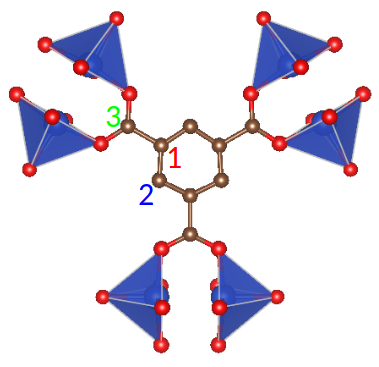
\includegraphics[width=0.65\textwidth]{hkust_molekula_placeholder.png}.
  \caption{}
\end{subfigure}%
   \begin{subfigure}[b]{0.5\textwidth}
  \centering
  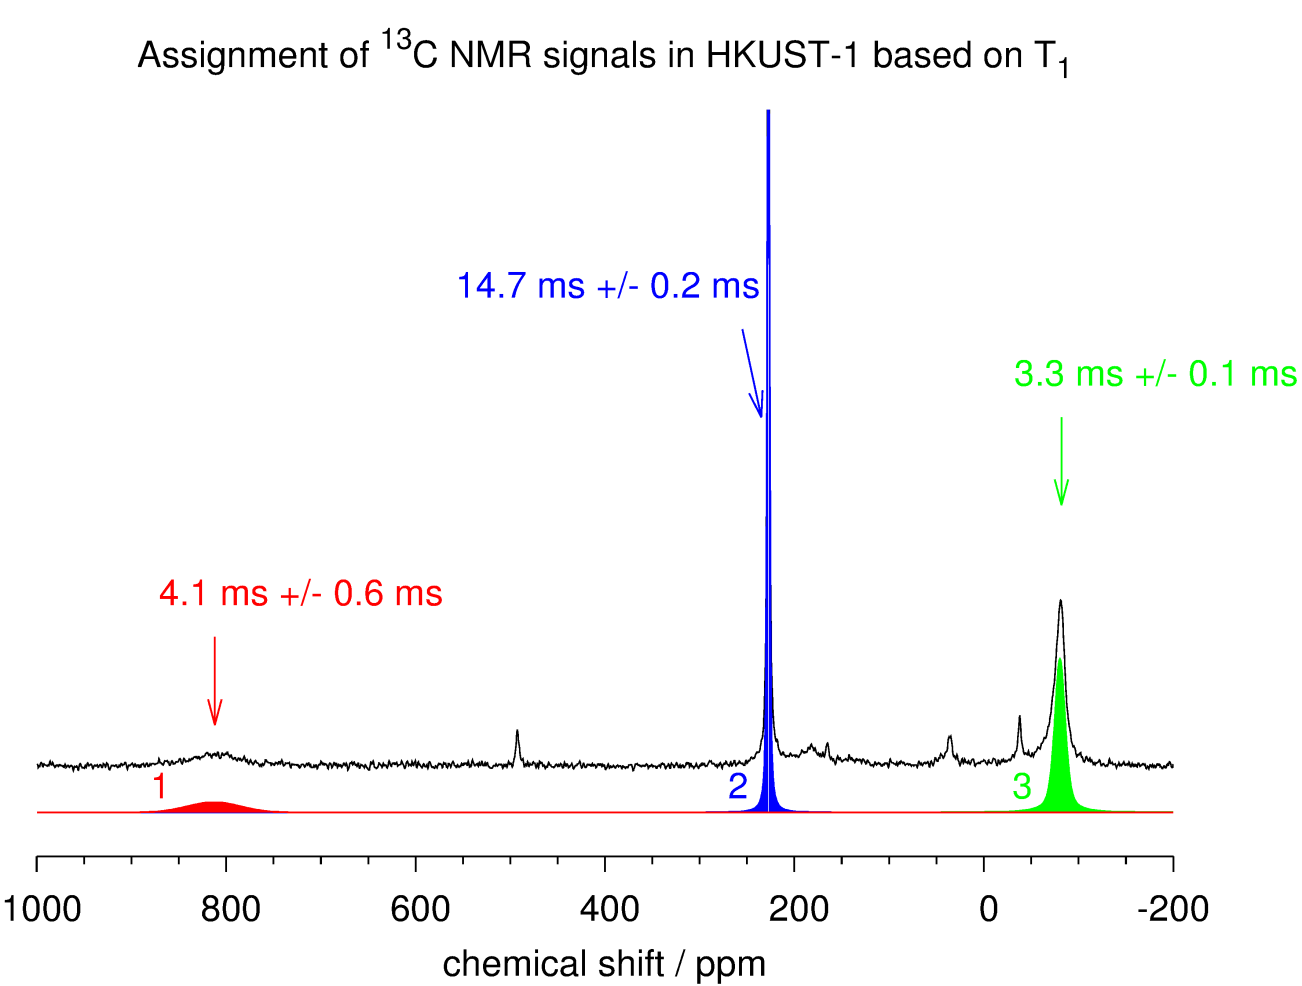
\includegraphics[width=0.9\textwidth]{hkust_spekter.png}.
  \caption{}
\end{subfigure}
  \caption{ An example of MOF named Hkust-1. It is a crystalline
    material. Image (a) depicts a part of the crystaline structure which is used for calculation of
    nmr parameters of atoms marked with 1, 2 and 3. (b) $^{13}\mathrm{C}$-nmr
    spectra of atoms marked on image (a).
  }
  \end{figure}

 Nmr spectra of organic materials usually feature chemical shifts caused by
 induced currents which in turn, are caused by external magnetic field
 \cite{chemic_shift_tensor_review}. In paramagnetic materials, this is not the
 only contribution to the total shifts visible in spectra. An important
 interaction, not present in  diamagnetic materials, is interaction between
 unpaired electrons and nuclei
 \cite{Dft_Investigation_of_the_Effect_of_Spin_Orbit}.
 Such interaction can cause large paramagnetic
 shifts also called hyperfine shifts. Typical for such spectra are also widened
 spectral lines. These large shifts make interpretation of spectra more difficult
 \cite{Dft_Investigation_of_the_Effect_of_Spin_Orbit}. A useful tool to help
 with the interpretation are first-principle quantum calculations. Large growth
 of computational power in recent years have enabled more accurate calculations
 and calculations performed on a more complex systems. However, calculations of
 hyperfine constants and total chemical shifts for paramagnetic materials / mofs
 have not yet been systematically tested and documented in literature.

 In this work we will present the most common approach to calculation of nmr
 parameters of paramagnetic materials,  which is based on density functional
 theory (dft). First we  will present basics of dft, which is the most important part of the whole procedure. Values of nmr parameters completely depend on electronic configuration, consequently it's accurate calculation is of a paramount importance. 

\section{Calculation of electronic wavefunction}
Accurate calculation of electronic structure has always been a challenge. It
quickly became apparent that direct use of Schr{\"o}dinger equation is not a
realistic prospect, except for some small
molecules, as the time consumed to solve it grows exponentially
\cite{nobel_lecture} as a function of electron
number at a given accuracy level. With the development of computers, different
numerical approximations for computation of electronic wave function and
optimization of molecular structure have emerged. One of the most successful methods has been density functional theory
(dft from now on), which has been known for roughly 50 years \cite{nobel_lecture}. Through the years dft has evolved and today it represents one of the main tools for calculation of electronic structure especially for complex molecules and crystals.

\subsection{Hamiltonian}
The first step in formulation of the problem is to define hamiltonian which
describes the motion of nuclei and electrons. Non-relativistic hamiltonian
describing the interaction of  nuclei and electrons can be written as follows:
\begin{equation} \label{full_hamiltonian}
\hat H= \hat T_n + \hat  T_e + \hat  W_{n-n} + \hat W_{e-e} + \hat W_{n-e} + \hat V_{ext},
\end{equation}
where $T_n$ and $T_e$ are kinetic energies of nuclei and electrons respectively,
$W_{n-n}$, $W_{e-e}$ and $W_{e-n}$ represent nuclei-nuclei, electron-electron
and electron-nuclei interaction terms. $V_{ext}$ is strictly multiplicative
external potential. Ground state of such a system is given by the solution of
the time independent Schr{\"o}dinger equation:
\begin{equation} \label{ham_solution}
\hat H \psi = \epsilon_0 \psi_0,
\end{equation} 
where index $0$ denotes the solution with the lowest energy. In general $\psi_0$
depends on $3N$ coordinates, where $N$ is total number of particles. This means
that systems with more than e.g. 10 atoms are very computationally
demanding. It is common practice to reduce the dimensionality of the problem by employing
Born-Oppenheimer approximation in which the motion of nuclei is separated from
the motion of electrons, sometimes their positions are even fixed
\cite{advanced_course, nobel_lecture}. Thus, from now on, we will
restrict ourselves to hamiltonians describing only the motion of electrons:
\begin{equation} \label{electron_hamiltonian}
\hat H=  \hat  T_e  + \hat W_{e-e} + \hat W_{n-e} + \hat V_{ext}.
\end{equation}
The number of electrons $N$ for a small molecules, like water, is of the order
$\sim 10$. In medium sized molecules with $\sim 50-100$ atoms, the number can
grow to a few hundred, while in large molecules, like proteins, the number can
grow into thousands and ten-thousands \cite{ab_initio_nmr_spect_molec}. As one can imagine, solving a system of
coupled differential equations with so large number of coordinates ($3N$) is
computationally an almost impossible task.
This is the reason for development of approaches which, while still being
sufficiently accurate, offer faster computational times. DFT represents one of
the most successful methods for solving such systems.

\subsection{Density functional theory - dft}
Dft allows us replaces all electron wave function with
electron density and effectively reduce the problem to a single electron problem.
The core of dft lies in Kohn-Sham theorems. These two theorems
ensure that stationary many-electron systems are fully characterized by their
ground state electron density. This means that given a group of electrons, one
only has to know ground state electron density to be able to tell all the other
properties of the system \cite{nobel_lecture}. For non-degenerate cases, the latter is uniquely
determined by the ground state many-electron wave function, which in turn is
uniquely determined by the external potential. For a simple non-degenerate case
we will prove these two theorems.
Let us consider hamiltonian of the form:
\begin{equation} \label{ks_hamiltonian}
\hat H = \hat T + \hat W + \hat V_{ext},
\end{equation}
where $T$ is kinetic energy, $W$ is inter-particle interaction and $V_{ext}$ is
external potential determined up to a constant. Let $V_{ext}$ be such a potential
that ground state $\psi_0$ is non-degenerate. Consider now the set of all $H$ of
the form (\ref{ks_hamiltonian}), which differ only in the $V_{ext}$, with
non-degenerate ground states. Since kinetic and inter-particle interaction terms
are the same for all $H$ in such a set, the latter can be represented by the set of all non-equivalent potentials:
\begin{equation}
  \begin{split}
    \mathcal{V} = \{V_{ext};\quad &\textrm{V determined up to a constant;}\\
    & \textrm{$\ket{\psi_o}$ exists and is non-degenerate}\}
    \end{split}
 \end{equation}
According to the above definition we can define the set of all corresponding
ground state-densities determined up to a phase as:
\begin{equation}
  \begin{split}
    \mathcal{G} = \{\psi_0; \quad &\textrm{$\psi_0$ ground state corresponding to external potential $V_{ext}$;}\\
&\textrm{ $\psi_0\sim\psi_0e^{i\phi}$   }
    \}
    \end{split}
  \end{equation}
The map from $\mathcal{V}$ to $\mathcal{G}$ is surjective by definition. What we
would like to know is, if it is also injective  (\ref{bijection}), i.e., can a
single $\psi_0$ be a ground state for two non-equivalent potentials? Suppose now
that $\psi_0$ is a ground state for two non-equivalent potentials $V_{ext}$ and $V'_{ext}$.

\begin{figure}[!ht]
  \centering
  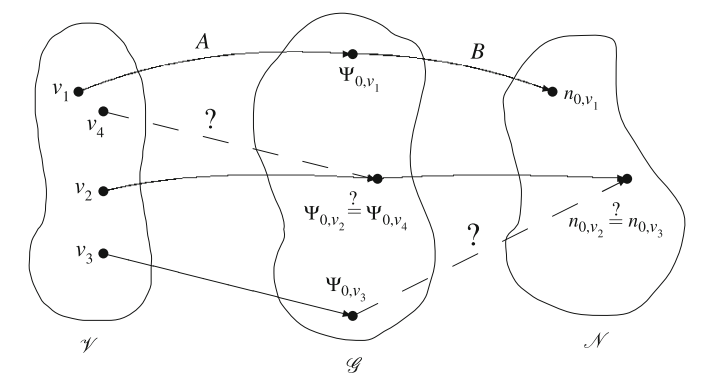
\includegraphics[width=0.6\textwidth]{bijekcija_med_v_psi_n.png}.
  \caption{Bijection between the set of potentials, the set of their corresponding ground
    states and the set of ground state densities. Existance of such bijection is proven by
    Kohn-Sham theorems and proves that many-particle system is
    uniquely determined by it's ground state particle
    density~\cite{advanced_course}.}
  \label{bijection}
\end{figure}

\begin{dgroup*}
\begin{dmath}
 \hat H\ket{\psi_0} =(\hat T + \hat W + \hat V_{ext}) \ket{\psi_0}\hiderel{=}\epsilon_0\ket{\psi_0}
\end{dmath},
\begin{dmath}
 \hat H'\ket{\psi_0} =(\hat T + \hat W + \hat V'_{ext}) \ket{\psi_0}\hiderel{=}\epsilon'_0\ket{\psi_0}
\end{dmath},
\begin{dsuspend}
subtracting above equation yields:
\end{dsuspend}
\begin{dmath}
(\hat V_{ext} - \hat V'_{ext})\ket{\psi_0}=(\epsilon_0-\epsilon'_0)\ket{\psi_0}.
\end{dmath}.
\begin{dsuspend}
 Due to multiplicative nature of potentials, we can just divide the whole
 equation by $\ket{\psi_0}$ and obtain: 
\end{dsuspend}
\begin{dmath}
  (\hat V_{ext} - \hat V'_{ext})=(\epsilon_0-\epsilon'_0),
  \end{dmath}
\end{dgroup*}
which is a contradiction, since $V_{ext}$ and $V'_{ext}$ must differ for more
than a constant. Similarly, one can show that two different ground state wave
functions, corresponding to two different external potentials, cannot lead to
the same ground state densities.  To see this, we compare ground state energies
and rewrite them using ground state densities, which are supposed to be the same
for both wave functions:

\begin{dgroup*}
\begin{dmath}
 \bra{\psi_o}\hat H\ket{\psi_0}=\epsilon_0 < \bra{\psi'_o}\hat H\ket{\psi'_0}=
 \bra{\psi'_o}\hat H + \hat V'_{ext} - \hat V'_{ext} \ket{\psi'_0}=\\ \epsilon'_0
 +  \bra{\psi'_o} \hat V_{ext} - \hat V'_{ext} \ket{\psi'_0}.
\end{dmath}
\begin{dsuspend}
 Rewriting this in terms of densities and taking into account equivalence of H
 and H' yields:
\end{dsuspend}
\begin{dmath}
\epsilon_0 <  \epsilon'_0 + \int (V_{ext}(\vec r)-V'_{ext}(\vec r))n(\vec r)
\dif \vec r
\end{dmath}
\begin{dsuspend}
  and
\end{dsuspend}
\begin{dmath}
\epsilon'_0 <  \epsilon_0 + \int (V'_{ext}(\vec r)-V_{ext}(\vec r))n(\vec r)
\dif \vec r.
\end{dmath}
\begin{dsuspend}
  Upon subtracting both equations one obtains a contradiction:
\end{dsuspend}
\begin{dmath}
  \epsilon_0 + \epsilon'_0< \epsilon_0 + \epsilon'_0,
\end{dmath}
\end{dgroup*}
which proves that for hamiltonians, which yield non-degenerate ground states,
each ground state leads to a different ground state electron density. Ground
state electron densities form a set where each density corresponds to a single
wave function from $\mathcal G$:
\begin{equation}
  \mathcal N = \left\{n; n=\bra{\psi_0}\hat n \ket{\psi_0}, \psi_0 \in \mathcal G \right\},
\end{equation}
where $\hat n$ is quantum mechanical electron density operator.

Extension of this simple proof to hamiltonians with degenerate ground states is
possible by replacing ground state wave functions by linear span of degenerate
ground states. Thus, in degenerate case one obtains bijection between external
potential, set of linear spans, each belonging to a certain external potential
and a set of sets of ground state densities. Special treatment is necessary also
for systems containing magnetic fields, where one can separate hamiltonian into
spin up and spin down hamiltonian of the form (\ref{ks_hamiltonian}). In the
latter case one obtains bijections between the set of pairs $(\vec A(\vec r),
V_{ext}(\vec r))$, $(\psi_\uparrow, \psi_{\downarrow})$ and $(n(\vec r), \vec m
(\vec r))$.

Since there exists bijection between ground state wave functions and ground
state densities, one can formally rewrite ground state wave function as
functional of ground state electron density:
\begin{equation}
  \ket{\psi'_0} =  \ket{\Psi[n'_0]}
  \end{equation}
and using above formula one can also rewrite operators in terms of ground state
density. As an example, let us rewrite ground state energy as functional of
ground state electron density:
\begin{equation} \label{hamiltonian_density}
  E[n_0] = \bra{\Psi[n_0]}\hat H \ket{\Psi[n_0]},
  \end{equation}

for which one can find minimum energy principle: $E[n_0]<E[n]$ whenever n
belongs to $\mathcal N$. This an obvious consequence of wave function functional
$\ket{\psi [n]}$, which is only defined for densities which are in $\mathcal N$.
Thus, one has to ask himself whether every nonegative normalizable function
$n(\vec r)$ is in $\mathcal N$.  The answer is no. A density from $\mathcal N$
have a corresponding potential $V_{ext}$ such that it minimizes energy functional
of the form \ref{hamiltonian_density} and consequently they are called V-representable densities. 

In practice, one does not need deep knowledge about such mathematical
definitions of functionals. The reason for this is the discretization of space
into grid points. On final grid for any strictly positive electron density
($n(\vec r) > 0$) there exists a potential for which the density represents ground state density and is thus contained in $\mathcal N$ \cite{advanced_course}.


  \section{DFT in practice}
Kohn-Sham theorems unfortunately tell nothing about the explicit dependence of
energy functional on density. Nonetheless, we would still like to use Kohn-Sham
theorems, to construct numerical scheme where electron density has the central
role. From now on will concentrate on construction suitable dft scheme and finding energy functional $E[n(\vec r)]$,
which should approximate $F[n(\vec r)]$ as well as possible.
  
  \subsection{Kohn-Sham equations}
  Kohn-Sham (KS) equations represent a standard and most common approach to dft.
  They are based on energy functional dependent only on electron density $n(\vec
  r)$. To introduce them in an understandable and consistent fashion, let's start with a non-interacting system. 
 
\subsection{Noninteracting system}
Hamiltonian of $N$-electron non-interacting system can be written in the
following way:
 \begin{equation} \label{noninteracting_H}
   \hat H =\hat  W_k + \hat V_{ext}, 
 \end{equation}
 where $V_{ext}$ is an external potential of multiplicative nature. It is well
 known that the solution to this problem can be written in the form of Slater determinant:

 \[
      \frac{1}{\sqrt{N!}}\det 
   \begin{bmatrix}
   \phi_{1}(\vec r_1, \sigma_1) & \phi_{2}(\vec r_1, \sigma_1) & \phi_{3}(\vec
   r_1, \sigma_1) & \dots & \phi_{N}(\vec r_1, \sigma_1) \\
    \phi_{1}(\vec r_2, \sigma_2) & \phi_{2}(\vec r_2, \sigma_2) & \phi_{3}(\vec
    r_2, \sigma_2) & \dots & \phi_{N}(\vec r_2, \sigma_2) \\
    \vdots & \vdots & \vdots & \ddots & \vdots \\
     \phi_{1}(\vec r_N, \sigma_N) & \phi_{2}(\vec r_N, \sigma_N) & \phi_{3}(\vec r_N, \sigma_N) & \dots & \phi_{N}(\vec r_N, \sigma_N) \\
\end{bmatrix},
\]
 which, when inserted into equation (\ref{noninteracting_H}) effectively produces
 single electron problem:
 \begin{equation}
   \left(-\frac{\hbar^2}{2m}\nabla^2 + \hat V_{ext}(\vec r)\right) \phi_i (\vec r) = \epsilon_i \phi_i(\vec r).
 \end{equation}
 Thus, using slater determinant we have effectively converted many electron
 problem with $3N$ coordinates to a single electron problem. Of course the
 electrons in this case do not feel each other and motion of each electron
 should not depend on other electrons, so such a breakdown is completely natural
 (except for Pauli principle which is already built into Slater determinant).
 
 The ground state of such a system is obtained using $N/2$ lowest states by
 putting $2$  electrons into each state. Calculation of kinetic energy and
 electron density for such a system is straight forward. As we can see,
 using Slater  determinant as ansatz for the solution of noninteracting
 hamiltonian offers simple expressions for ground state wavefunction, kinetic
 energy and electron density  calculation. Electron density corresponding to
 such a wave function can be written using the following expression:
 \begin{equation} \label{KS_density}
   n_0(\vec r) = \sum_{\sigma=\uparrow,\downarrow}\sum_i\Theta(\epsilon_F-\epsilon_i)|\phi_i(\vec r, \sigma)|^2.
 \end{equation}
 The density of electrons is just a sum over all occupied orbitals. Now let's
 remember Kohn-Sham theorems, which state that ground state density is unique
 functional of the ground state wave function:
 \begin{equation}
   \ket{\psi(\vec r)}= \ket{\Psi[n(\vec r)]}.
 \end{equation}
 One can show that there exists an even stronger connection; every $\phi_i$ is a
 uniquely determined by ground state density. One can see this by considering a single electron problem using the same potential $V_{ext}$ as found in eq.
 (\ref{noninteracting_H}) and then gradually adding electrons, thus:
 \begin{equation}
   \ket{\phi_i(\vec r)}= \ket{\Phi_i[n(\vec r)]}.
 \end{equation}
 Using this relations we can define HK functional:
 \begin{equation}
   E_s[n(\vec r)] = \bra{\Psi[n(\vec r)]}T \ket{\Psi(n(\vec r))} + \int n(\vec r) V_{ext}(\vec r)  \dif \vec r,
   \end{equation}
 where
\begin{equation} \label{KS_kinetic_term}
   T[n(\vec r)] = \sum_i\Theta(\epsilon_F-\epsilon_i)  \sum_{\sigma=\uparrow,\downarrow}\int \phi^*_\sigma(\vec r)\frac{-i\hbar\nabla^2}{2m}\phi_\sigma(\vec r),
 \end{equation}
 where we have implicitly used $\ket{\phi_i(\vec r)} = \ket{ \Phi_i[n(\vec r)] }$.
 In practice this in not necessary, since functions $\phi(\vec r)$ are known.
 
Now we would like to use a similar construction to solve hamiltonian
\ref{hamiltonian_density}. Using solution ansatz in the form of Slater
determinant offers straight forward calculation of kinetic energy and electron
density. Using Slater determinant leads to differential equations for $\phi_k$
wavefunctions. Modern computational packages instead of solving differential
equations use large sets of basis functions, which in the end lead to
eigenvalue problem. Solution is then given by populating
lowest energy orbitals until all electrons are allocated.

To solve interacting system using dft one relies on the fact, that for every
interacting hamiltonian with ground state density $n_0$, there exists
noninteracting hamilotnian with exactly the same ground state density \cite{advanced_course}.
This fact still does not tell us what kind of external potential
one should use to produce the same electron density.

Intuitively, one would expect that potential belonging to effective single
electron hamiltonian should reflect the properties, geometry and potentials found
in a given interacting system. Hamiltonian naturally contains kinetic energy
term, but it should also somehow contain inter particle interactions. Usually
Kohn-Sham hamiltonian consists of kinetic energy term, Hartree inter particle
interaction, external potential and exchange-correlation functional \cite{advanced_course}:
\begin{equation} \label{KS_system}
  E[n(\vec r)]=T[n(\vec r)]] + E_H[n(\vec r)]] + E_{ext}[n(\vec r)]] + E_{xc}[n(\vec r)]].
\end{equation}
Hartree term accounts for Coulomb repulsion:
\begin{equation} \label{hartree_term1}
  E_H[n(\vec r)] = \int n(\vec r)w(\vec r, \vec r') n(\vec r')\dif \vec r' \dif \vec r.
\end{equation}
The above expression is not the same as the one we get from Hartree-Fock
equations and includes self-repulsion. Dft treats exchange term, also arising
from Coluomb potential, separately. Computational packages often employ different
approximation and optimizations for faster calculation of this term \cite{orca}.
Functional belonging to external potential is well known: 
\begin{equation} \label{ext_potential_functional}
  E_{ext}[n(\vec r)] = \int n(\vec r) V_{ext}(\vec r) \dif \vec r.
\end{equation}
Unfortunately exchange-correlation functional is much less well known. It is
defined by the equation (\ref{KS_system}) and contains all the inter-particle
interactions not contained in $T[n(\vec r)]$ and $ E_H[n(\vec r)]]$. It is
common to divide $E_{xc}[n(\vec r)]$ into exchange $E_x[n(\vec r)]$ and
correlation $E_c[n(\vec r)]$ part. The former is defined in such a way that
Hartree-Fock ground state density and energy are reproduced, if correlation part
is neglected. This is achieved if exchange part of functional has exactly the
opposite contribution as excessive hartree term in KS equations: 

\begin{equation}
  E_{x}[n(\vec r)]=-\frac{1}{2}\sum_{k,l}\Theta(\epsilon_F-\epsilon_k)\Theta(\epsilon_F-\epsilon_l)\int \dif \vec{r} \dif \vec{r'}\phi^*_k(\vec r, \sigma)\phi_l(\vec{r}, \sigma)w(\vec{r},\vec{r'})\phi^*_l(\vec{r'}, \sigma')\phi_k(\vec{r'}, \sigma')
\end{equation}
The most important contribution of $E_{x}[n(\vec r)]$ is cancellation of
self-repulsion. This term is commonly called exact exchange and is not always
used in dft calculations. Exchange functionals based only on
electron density are often employed and they do not manage to completely cancel
self-repulsion terms. We will take a closer look at them in the following chapter.
Correlation term is more difficult to derive and we will not dwell deeper into
it. Instead let's have a look at how KS equations are actually solved.

Our goal is to minimize hamiltonian of the form (\ref{KS_system}) using Slater
determinant as ansatz for many electron system and density calculation. By
considering (\ref{ext_potential_functional}) and (\ref{KS_kinetic_term}) one can
write KS equation:  
\begin{equation}
  \left( \hat T + v_{ext} + E_H[n(\vec r)]]  + E_{xc}[n(\vec r)]] \right) \ket \phi_i =  \epsilon_i \ket{\phi_i},  
\end {equation}
where density $n(\vec r)$  has to be calculated according to equation
(\ref{KS_density}). They are usually determined by inserting ansatz in the
form of gaussian basis functions from which one can
then construct correct single electron states. Multiplying equation by $\bra
\phi_j$ from the left side yields generalized eigenvalue problem:
\begin{equation}
  \bra {\phi_j} \left( \hat T + v_{ext}(\vec r) + E_H[n(\vec r)]]  + E_{xc}[n(\vec r)]] \right) \ket{\phi_i} =  \epsilon_i \braket{ \phi_j |\phi_i }.
\end {equation}

System obviously has to be solved in a self consistent fashion
(fig. \ref{self_consistent_scheme}). One starts with the positioning of nuclei into
desired positions and construction of nuclei potentials. In parallel with the
last step starting electron orbitals $\phi^{(0)}_i$ are constructed. Usually they are written
as a series of Gaussian functions. Electron density $n^0$ can then be quickly
calculated from constructed orbitals. After that one
calculates functionals $E_H[n(\vec r)]$ and $E_{xc}[n(\vec r)]$. In the next step
equations are solved. The solution are new orbitals $\phi_i^{(1)}$  and from
them, the new density $n^{(1)}$ is calculated. The latter is then used to construct new $E_H[n(\vec r)]$ and $E_{xc}[n(\vec r)]$ which are again used to
solve KS equation from which one gets new orbitals $\phi^{(3)}$. The procedure is
repeated until the change in density or energy is not small enough. 


\begin{figure}
  \centering
  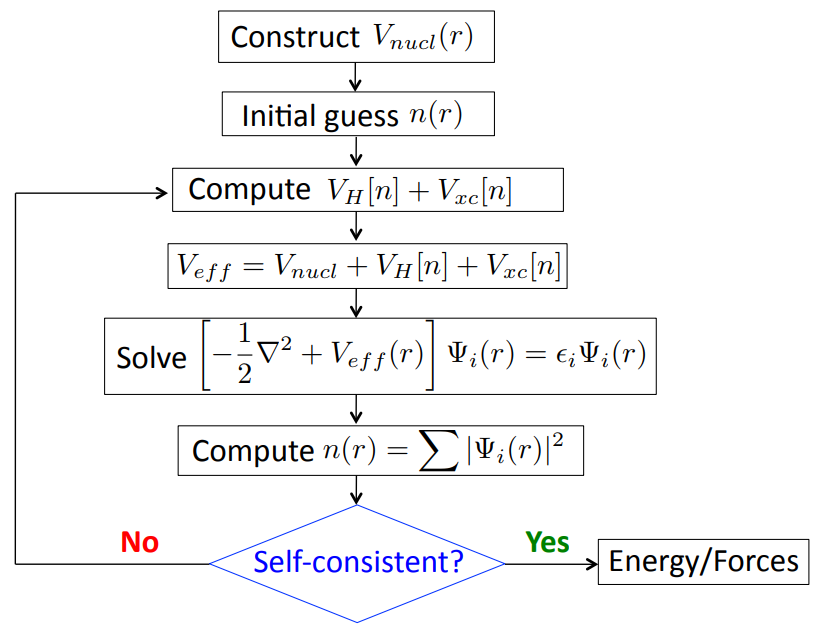
\includegraphics[width=0.65\textwidth]{self_consistent_scheme.png}.
  \caption{Self consistent scheme depicting the procedure in which Kohn Sham
    equations are solved. One starts with the positioning of nuclei into
    desired positions. The next step is to construct potential of nuclei and in
    parallel one can also construct starting approximation for electronic wave
    function. The latter is then used for constructing all other functionals of
    density. After all functionals have been established one can solve KS
    equations, construct new density and repeat the described procedure until
    the change in density is not small enough.
  }
  \label{self_consistent_scheme}
\end{figure}

When given a certain system, functionals $T$, $E_H$ and $V_{ext}$ are precisely
determined. $E_{xc}$ is not. It is thus the determining factor for how well the KS
equations describe our system. We will present various functionals used today in
one of the next chapters.

\subsubsection{Degenerate ground state}
So far we have talked little about the problem of degeneracy of KS states. In
general degeneracy is not a problem, except at Fermi level. When there are more
KS states than there are electrons, several possible ground states and thus also
electron densities can be constructed. In such cases density matrix arising from
several Slater determinants is constructed \cite{advanced_course}:
\begin{equation}
  \hat D = \sum_i d_i\ket{\Phi_i} \bra{\Phi_i}.
  \end{equation}
Density belonging to such ground state is just a weighted sum of densities
corresponding to each Slater determinant $n(\vec r)=\sum_id_in_i(\vec r)$, where
$n_i(\vec r)=\sum_j|\phi_{ij}(\vec r)|^2$. Index $i$ runs over all possible
Slater determinants one can construct from given degenerate states and index $j$
runs over all states in each Slater determinant. The sum of coefficients $d_k$
is the trace of density matrix and has to be $1$. The choice of coefficients
$d_k$ is not trivial. They have to be constructed in such a way that the new
electron density does not break degeneracy. When a new degenerate state emerges in
scf procedure (fig. \ref{self_consistent_scheme}), it may significantly affect
electron density and resulting potentials and consequently break or destroy
convergence of the procedure. An example is a boron atom where 2p orbitals are
degenerate. Only the choice of $d_{2p^0}=d_{2p^{-1}}=d_{2p^1}=1/3$ leads to spherically symmetric potential and preservation of degeneracy\cite{advanced_course}.

\subsection{Exchange and correlation functionals}
Exchange and correlation functionals are functionals which try to account for
exchange and correlation interactions between electrons. They can be of a
different forms and in general one can roughly divide them into 4 groups
\cite{challenges_den_fun_theor, presc_desig_selec_densit_funct_approx}: Lda, Gga, meta-Gga and Hybrid functionals.
The first three groups all have in common that they explicitly depend on density
of electrons. This causes a self-interaction error, which causes excessive
delocalization of electrons. As a solution to these problems hybrid
functionals, which contain exact Hartree-Fock exchange, have been proposed.

\subsubsection{Lda}
Local density approximation (lda) are functionals which depend only on
 electron density \cite{challenges_den_fun_theor, presc_desig_selec_densit_funct_approx}.
First functional of such form dates back into
the year 1930, when the exchange interaction for uniform gas was discovered
\cite{challenges_den_fun_theor} :
\begin{equation} \label{electron_gas_exchange}
E_{xc}^{lda}[n]=-\frac{3}{4}\left( \frac{3}{\pi} \right)^{1/3}\int n(\vec r)^{4/3} \dif \vec r.
\end{equation}
The correlation part has not been derived, but it is accurately known from Monte
Carlo simulations \cite{presc_desig_selec_densit_funct_approx}.
Today, there exist multiple other lda exchange--correlation functionals, but for most cases
they are not very useful. Their only advantage are fast computational times.
For every other purpose gga and hybrid functionals are much better suited.

\subsubsection{Gga}
Generalized gradient approximation (gga) functionals
depend not only on electron density but also on its gradient
\cite{challenges_den_fun_theor}. Most commonly, gga functionals are build upon (\ref{electron_gas_exchange}) \cite{challenges_den_fun_theor}:
\begin{equation}
  E_{xc}^{gga}=\int n(\vec r)^{4/3}F(x);\quad x=|\nabla n(\vec r)|/n(\vec r)^{4/3}.
\end{equation}
One of most commonly used gga functional is PBE functional
\cite{challenges_den_fun_theor} \cite{challenges_den_fun_theor}:
\begin{equation}
  E_{xc}^{pbe}=-\int  n(\vec r)^{4/3}\left[ \frac{3}{4}\left(\frac{3}{\pi}\right)^{1/3} + \frac{\mu s}{1+ \mu s^2/\kappa} \right]; \quad s=x/(2(3\pi/2)^{1/3}).
\end{equation}
Gga functionals offer acceptable accuracy and fast computational times and are
most commonly used for approximate calculations, before starting more accurate
and more time consuming calculations using hybrid or meta-gga functionals.

\subsubsection{Meta-gga functionals}
Since gga functionals have their short commings, meta-gga functionals were formed
in belief that adding higher derivatives will improve accuracy
\cite{challenges_den_fun_theor}. Meta-gga functionals are build upon gga
functional form and add terms containing higher order derivatives of electron
density. Functionals are formulated according to the following equation
\cite{challenges_den_fun_theor}:

\begin{equation}
  E_{xc}^{MGGA}= \int \rho^{4/3}F(\rho(\vec r) \nabla \rho(\vec r), \nabla^2 \rho(\vec r), \tau(\vec r)); \quad \tau=\frac{1}{2}\sum_i |\nabla \phi_i(\vec r)|^2
   \end{equation}

Meta-gga functionals have higher computational cost than gga functionals.
Unfortunately, as it turned out, they are not significantly better than gga
functionals and are thus not so popular.


\subsubsection{Hybrid functionals}
On the contrary to meta-gga functionals, hybrid functionals are much more
successful \cite{challenges_den_fun_theor}. These functionals are not a
continuation of lda, gga, meta-gga chain. Instead, they incorporate exact
Hartree-Fock exchange term \cite{challenges_den_fun_theor}:
\begin{equation}
  E^{hf}_{xc}=\sum_ {i,j,\sigma}\int\frac{\phi^*_{i\sigma}(\vec r) \phi_{j\sigma}(\vec r) \phi^*_{j\sigma}(\vec r') \phi_{i\sigma}(\vec r')}{|\vec r - \vec r'|}\dif \vec r \dif \vec r'.
\end{equation}
Such functionals do not break Kohn Sham formalism since the wave functions
$\phi_i(\vec r)$ are unique functional of densities shown in previous chapter.


\begin{figure}[!ht]
  \centering
  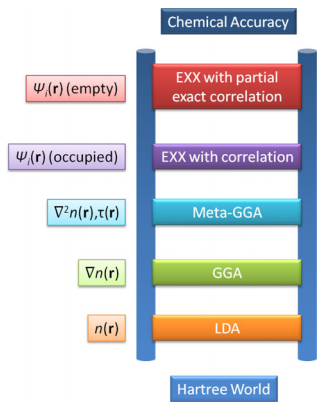
\includegraphics[width=0.4\textwidth]{jacobs_functional_ladder_ver2.png}.
  \caption{Jacob’s ladder of exchange-correlation functional approximations
    employed in dft calculations. Hartree world represents starting level where only
    weak interparticle interaction is present. Lda approxiamtion covers
    functionals which depend only on electron density. Gga additionally depends
    on gradient of electron density, while mega-gga incorporates higher order
    derivatives of electron density and in some cases even kinetic energy of
    orbitals ($\tau$). Hyper-gga functionals, also called hybrid functionals,
    stage represents functionals which contain exact exchange calculation (i.e.
    the one found in Hartree-Fock method). The last level utilizes all Kohn-Sham
    orbitals to calculate correlation and exchange interaction. This level also
    accounts for VdW interaction, which is caused by charge fluctuations and is
    not accounted for in previous stages \cite{How_theo_simul_can_address}.
  }
  \label{bijection}
\end{figure}

\subsection{Van der Waals dispersion}
Dft does not take into account effects caused by charge fluctuations. These Van
der Waals effects can be taken care of with different methods.
 The most promising seems to be the so called DFT-D method
\cite{consis_accur_ab_initio_param}, which is just a sum of terms $CR^{-6}$
over all atom pairs. As it is generally known, for large distances Van der Waals
potential should decay as $R^{-6}$ and this interaction does fulfill this condition.


\section{All electron vs pseudopotential}
Electronic states of an atom can be divided into three categories: core states,
semi-core states and valence states. The latter are the most actively included
in formation of bonds. Valence states may be completely deformed once the atom
is put into molecules/crystals. Semi-core states are states which do not
directly contribute to bonding, but may still be polarized or spatially
deformed. Lastly, core states, are highly localized and are assumed to be
unaffected by chemical bonding. This means that there should be very little loss
of accuracy, if core states are replaced by a pseudo wavefunction.
Pseudo potentials are constructs which try to
replicate effects of core electrons exerted on semi-core, valence electrons and
thus reproduce the correct chemical and physical properties (bonding energy, bond
length, electron localization, magnetization,...).

Of course, pseudo potentials have to be constructed prior to a given calculation using
some other much simpler system. As a consequence, there
exists a question of transferability. Is a potential constructed using some
reference molecule usable for another molecule. The exact answer is
not possible. Many times the only way is to try, especially when transition
elements are in question.

All electron calculations avoid pseudopotential by taking into account all
electrons. The latter does cost some computational time, but depending on the
molecule, it may be the only way to get reliable result. Of course for large
molecules all electron calculations are significantly more expensive.
Commonly used open source packages offering both approaches are Orca and Nwchem.


\section{Nmr parameters}
The two most important nmr quantities are shielding tensor and hyperfine tensor.
The former is important in all organic materials, while the latter is present
only in materials with unpaired electrons. Shielding tensor is 
proportionate to electron density at the observed  core site, whereas hyperfine
tensor is proportionate to the shielding tensor.


\begin{wrapfigure}{R}{0.4\textwidth}
\centering
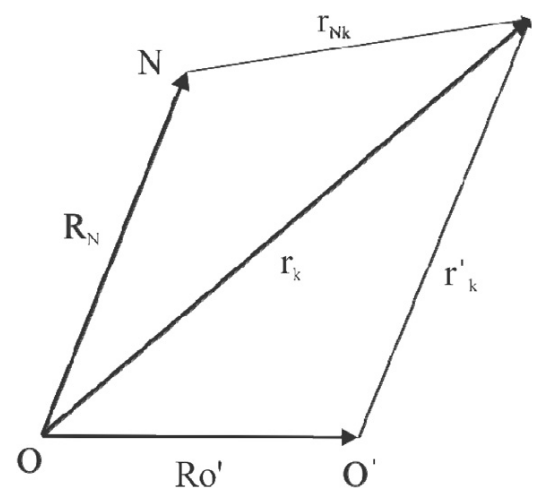
\includegraphics[width=0.3\textwidth]{origin_dependance_tensor.png}
\caption{Translation of the coordinate system for vector $\vec{Ro'}$. $\vec{R_N}$
  points to $N$-th atom, whereas small case $\vec r$ point to electrons.}
\end{wrapfigure}

  There are two contributions to the shielding tensor - paramagnetic and
  diamagnetic. The former is only present in materials with unpaired electrons
  and should not be confused with hyperfine tensor, also present in such materials.
  Diamagnetic contribution can be, in the first order of perturbation, calculated as \cite{chemic_shift_tensor_review}:
  \begin{equation}
    \sigma^d_{\alpha \beta}=\bra{\psi_0}\vec{r}_k \vec{r}_{Nk}\delta_{\alpha\beta}- \vec{r}_{k}\vec{r}_{Nk} \ket{\psi_0}
  \end{equation}
  and a similar expression holds also for paramagnetic contribution $\sigma^p_{\alpha\beta}$. Both
  expressions are nonlinear in $\vec r$. This seems to suggest that the values
  depend on the origin. It turns out, that the sum of both contributions does
  not depend on the origin, but only when one uses complete set of basis functions,
  which, in practice, is almost never the case. This is a serious problem
  because the terms that should theoretically cancel out have nontrivial
  contribution \cite{chemic_shift_tensor_review}. The issue is exaggerated by
  the fact that diamagnetic and paramagnetic contributions are of a different
  perturbation order.

  In constrast to shielding tensor which depends only on electron density,
  hyperfine tensor depends on spin density \cite{calcul_hyper_tensor_param_nmr}:
  \begin{equation}
    A_{iso}=\frac{4\pi}{6c^2}g_eg_N\beta_N\langle S_z \rangle \rho^{beta-alpha}(0),
    \end{equation}
where $g_e$ and $g_n$ are electronic and nuclear g-factors, $\langle S_z
\rangle$ is the expectation value of z component of total spin.  $\rho^{beta-alpha}$ is the difference between spin up and spin
down electron densities.

\section{Conclusion}
In this paper we tried to provide a clear and comprehensive review of steps needed
to calculate nmr parameters. The single most important step is accurate
calculation of electronic wave function. The latter is most commonly calculated
using dft, which has been in use for a long time and is still actively evolving.
Popular computational packages offer large variety of functionals, which are
suitable for numerous systems and their property calculations. 

\newpage \phantomsection


\addcontentsline{toc}{section}{Literatura}
\bibliographystyle{../myapsrevSLO}
\bibliography{../mybib}

\end{document}